\section{Indekser}
\subsection*{Hvorfor indekser?}
\begin{frame}{Indekser}
    \begin{itemize}[<+->]
        \item Rows er ikke sortert
        \item $\rightarrow$ finne informasjoner med WHERE tar tid
        \item Indekser er ekstrastrukturer som forenkler søking i tabeller
        \item Kan være en eller flere spalter
        \item Indekser funker som ordbok/lookup table
        \item Ulempe: De tar plass, må oppdateres
        \item To typer indekser:
            \begin{itemize}
                \item B-trær
                \item Hashing
            \end{itemize}
    \end{itemize}
\end{frame}

\subsection*{B-trær}
\begin{frame}{B-trær}
    \begin{itemize}
        \item innhold
    \end{itemize}
\end{frame}

\subsection*{Hashing}
\begin{frame}{Hashing}
    \begin{itemize}
        \item innhold
    \end{itemize}
\end{frame}

\subsection*{Eksempel}
\begin{frame}{Hvilke indeks skulle man ha?}
    \begin{itemize}
        \item innhold
    \end{itemize}
\end{frame}

\subsection*{Spørretid}
\begin{frame}{Spørsmål?}
    \begin{figure}
        \centering
        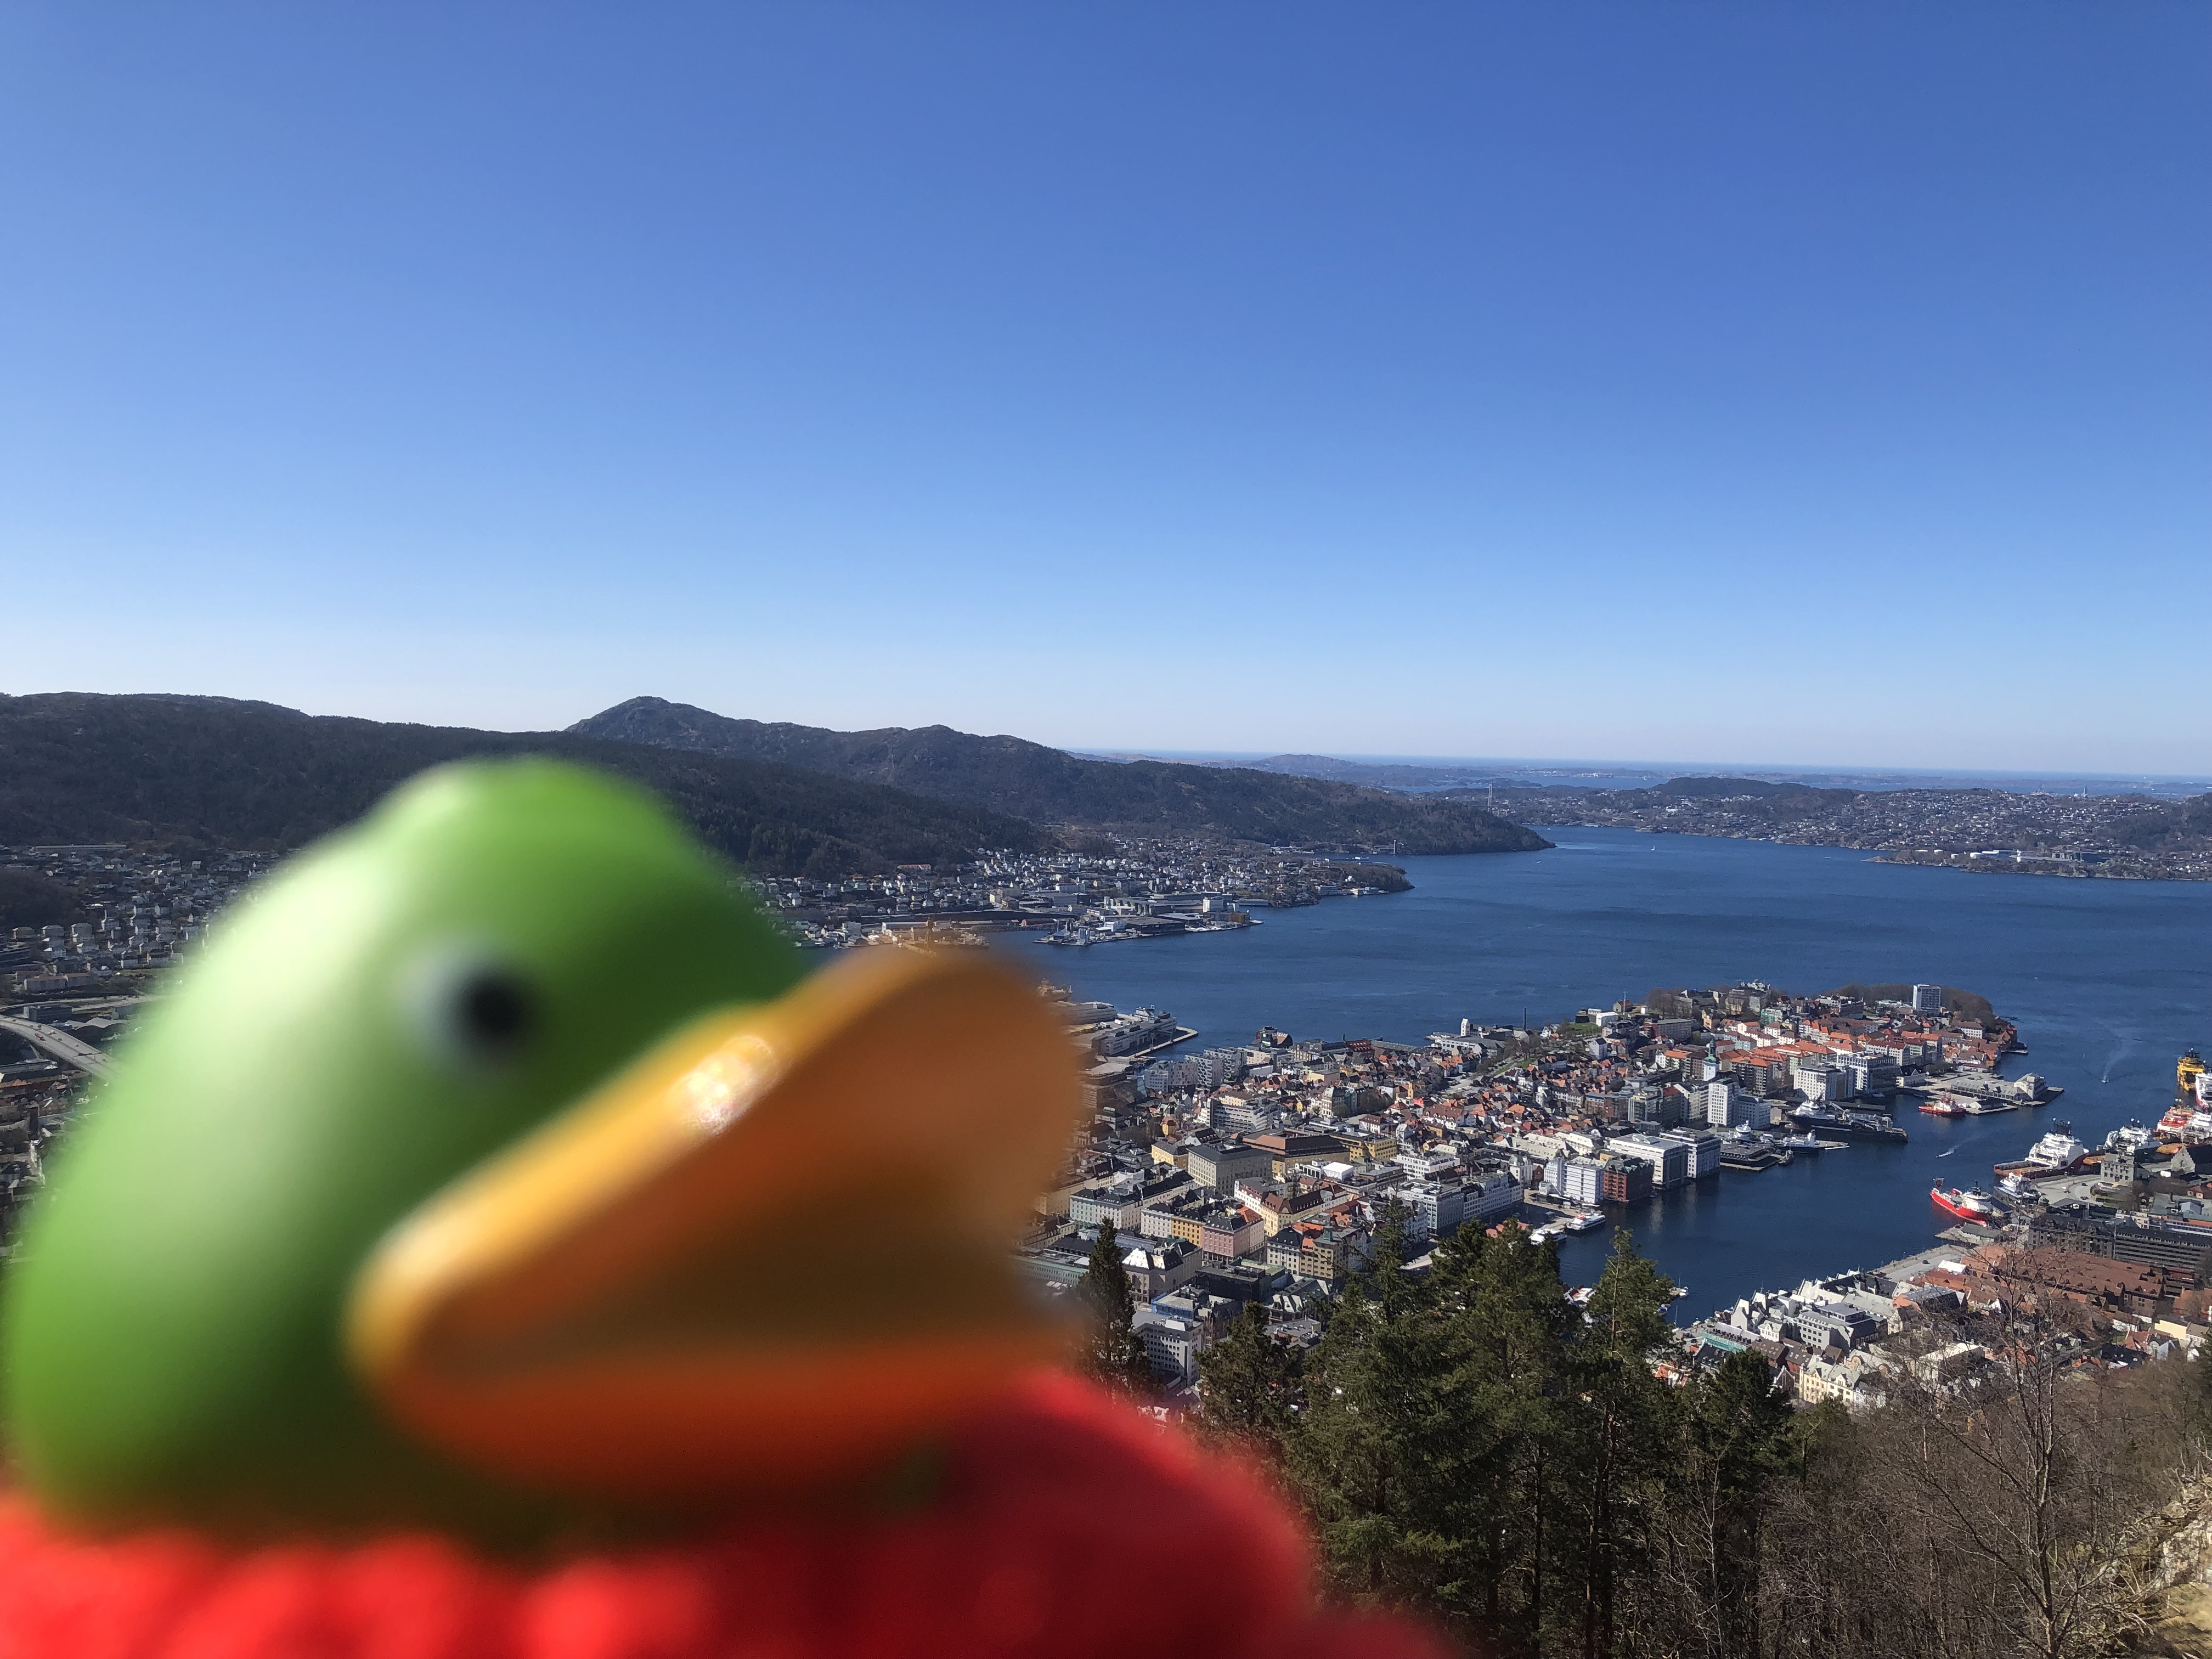
\includegraphics[height = 4.9cm]{images/guillaume10.jpg}
        \caption{Guillaume på Fløyen}
        \label{fig:guillaume10}
    \end{figure}
\end{frame}